\subsubsection{Memoria SD}

Las memorias SD (\textit{Secure Digital}) son dispositivos de almacenamiento de datos que han ganado popularidad debido a su tamaño compacto, capacidad de almacenamiento y facilidad de uso. Son ampliamente utilizadas en diversas aplicaciones, desde cámaras digitales hasta sistemas embebidos, gracias a su versatilidad y eficiencia. En la figura \ref{fig:sd_card} se visualiza una memoria SD.\\


\begin{figure}[H]
    \centering
    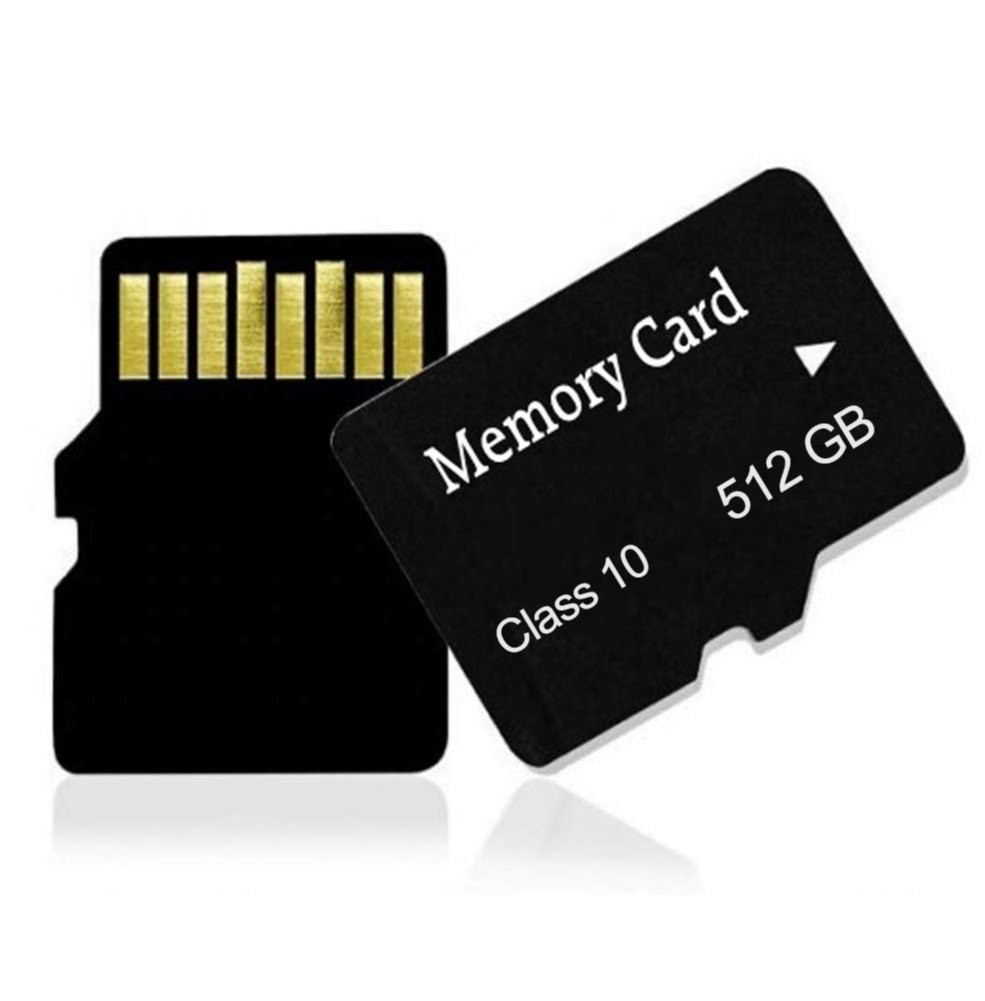
\includegraphics[scale = 0.2]{img/sd_card.jpg}
    \caption{Memoria SD}
    \label{fig:sd_card}
\end{figure}



Las memorias SD cuentan con las principales características: 
\begin{itemize}
    \item \textbf{Capacidad de almacenamiento}: las memorias SD están disponibles en varias capacidades, que varían desde unos pocos megabytes hasta varios terabytes. Esto permite a los usuarios elegir la memoria adecuada según sus necesidades específicas de almacenamiento.
    \item \textbf{Velocidades de transferencia}: existen diferentes clases de memorias SD, como Clase 2, 4, 6, 10, y UHS-I y UHS-II, que determinan la velocidad mínima de lectura y escritura. Las memorias de clase más alta son ideales para aplicaciones que requieren una rápida transferencia de datos, como la grabación de video en alta definición.
    \item \textbf{Interfaz de comunicación}: Las memorias SD utilizan una interfaz estándar que permite la conexión con dispositivos a través de protocolos como SPI (\textit{Serial Peripheral Interface}) o SDIO (\textit{Secure Digital Input Output}). Esto facilita su integración en una variedad de sistemas.
    \item \textbf{Durabilidad y fiabilidad}: muchas memorias SD están diseñadas para resistir condiciones adversas, como temperaturas extremas, golpes y vibraciones. Esto las hace adecuadas para su uso en entornos donde la robustez es fundamental.
    \item \textbf{Facilidad de uso}: la implementación de memorias SD es sencilla, ya que muchos dispositivos y plataformas de desarrollo ofrecen bibliotecas y herramientas que facilitan la lectura y escritura de datos en estas memorias.
\end{itemize}


En los sistemas embebidos las memorias SD se colocan sobre un zócalo que permite removerlas para luego insertar la memoria SD en una PC y descargar los datos, formatearla o repararla. También existen módulos para Arduino que permiten integrar una memoria SD al proyecto en etapas tempranas antes de fabricar un PCB propio y soldar un zócalo. Esto facilita mucho el mantenimiento y el desarrollo de sistemas que contienen almacenamiento de datos en memorias SD. \\

Existen tres formatos principales de memorias SD: SD estándar (32 x 24 mm), miniSD (21.5 x 20 mm) y microSD (15 x 11 mm). La microSD\textbf{ }es la más compacta y comúnmente utilizada en aplicaciones embebidas por su tamaño reducido y gran capacidad de almacenamiento. Por estos motivos, se utiliza el formato de memoria microSD para este proyecto. \\

Las memorias SD se han convertido en una solución de almacenamiento clave en muchos dispositivos electrónicos, ofreciendo una combinación de flexibilidad, capacidad y rendimiento que se adapta a una amplia gama de aplicaciones. 